\section{Metodologia}

\begin{frame}{Metodologia: Análise e Técnicas}
      \textbf{Estudo da Literatura:}
             \begin{itemize}
                 \item Nenhum trabalho similar encontrado em bases acadêmicas
             \end{itemize}

\begin{table}[H]
\scriptsize
  \caption{\tiny Resultados das bases após aplicar os critérios.}
\label{tab-result}
\begin{tabular}{l|c}
\scriptsize
  %\hline
   \textbf{Bases}  & \textbf{Filtrados}\\
   \hline
    IEEE Xplore Digital Library
    % NOTE: Eram 2, mas removi 'Tree-Structured Shading Decomposition'.
    % NOTE: Decidi voltar para 2 e incluir novamente o artigo removido
   & 2
    \\ \hline
    BDTD
    & 0
    \\ \hline
    CAPES Periódico
    & 0
    \\ \hline


  ACM Digital Library
  & 1
    \\ \hline
 Google Acadêmico
  & 1
   % \hline
\end{tabular}
\end{table}
       
      \textbf{Estudo Realizado} nas seguintes áreas:
             \begin{itemize}
                 \item Radiometria e BRDFs. Base teórica pelo livro ''Physically Based Rendering`` \cite{pbr}.
                 \item Linguagem de shader GLSL
                 \item Técnicas de análise sintática (Pratt Parsing) e geração de código
                 \item Análise de BRDFs existentes (Artigos)
             \end{itemize}

\end{frame}

\begin{frame}[fragile]{Metodologia: Design Inicial de Casos de Teste}
    Design inicial para validação da tradução BRDF em \LaTeX{} $\to$ GLSL\footnote{\tiny{Alguns símbolos não estão definidos para simplificar}}

   { \small
   \begin{equation*}
       \text{cook\_torrance}(\omega_i, \omega_o) = \frac{D(h)F(\omega_i, h)G(\omega_i, \omega_o, h)}{4(\omega_i \cdot n)(\omega_o \cdot n)}
   \end{equation*}
   }

    \vspace{1cm}
   \begin{columns}
       
       % Coluna do código LaTeX
       \column{0.5\textwidth}
       \LaTeX{} Fonte
       \begin{lstlisting}[basicstyle=\scriptsize]
\text{cook\_torrance}(\omega_i, \omega_o)
   = \frac{D(h)F(\omega_i, h)G(\omega_i,
   \omega_o, h)}{4(\omega_i \cdot n)
   (\omega_o \cdot n)}
       \end{lstlisting}
       
       % Coluna do GLSL
       \column{0.5\textwidth}
       GLSL a ser gerado
       \begin{lstlisting}[language=C, basicstyle=\tiny]
vec3 cook_torrance(vec3 wi, vec3 wo) {
   float D_RESULT = D(h);
   vec3  F_RESULT = F(wi, wo);
   float G_RESULT = G(wi, wo, h);
   float den = 4.0 * dot(n, wi) * dot(n, wo);
   return D_RESULT * F_RESULT * G_RESULT / den;
}
       \end{lstlisting}
   \end{columns}
   
   % \vspace{0.3cm}

\end{frame}

\begin{frame}{Metodologia: Implementação do Compilador}
   \begin{columns}
       % Coluna de texto principal
       \column{0.65\textwidth}
       \begin{itemize}
           \item \textbf{Linguagem Odin:}
                 \begin{itemize}
                     \item Linguagem de propósito geral, orientada a dados
                     \item Sem dependências externas (biliotecas padrão)
                 \end{itemize}
           \item \textbf{Etapas do Compilador:}
                 \begin{itemize}
                     \item Lexer e Parser (Pratt Parsing)
                     \item Análise Semântica (checker)
                     \item Travessia AST (walker)
                     \item Geração GLSL (emitter)
                 \end{itemize}
       \end{itemize}
       
       % Coluna da direita com diagrama simples
       \column{0.35\textwidth}
       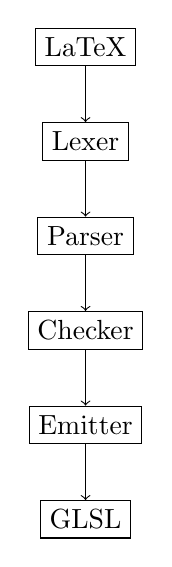
\begin{tikzpicture}[node distance=1.2cm]
           \node[draw] (latex) {LaTeX};
           \node[draw, below of=latex] (lexer) {Lexer};
           \node[draw, below of=lexer] (parser) {Parser};
           \node[draw, below of=parser] (checker) {Checker};
           \node[draw, below of=checker] (emitter) {Emitter};
           \node[draw, below of=emitter] (glsl) {GLSL};
           
           \draw[->] (latex) -- (lexer);
           \draw[->] (lexer) -- (parser);
           \draw[->] (parser) -- (checker);
           \draw[->] (checker) -- (emitter);
           \draw[->] (emitter) -- (glsl);
       \end{tikzpicture}
   \end{columns}
\end{frame}

\begin{frame}[fragile]{Metodologia: Especificação da Linguagem}
    Subconjunto do ambiente equation (\verb|\begin{equation}|) essencial para descrever BRDFs
\begin{table}
\centering
    \scriptsize % or \footnotesize or \scriptsize
\begin{tabular}{l|l|l}
% \begin{tabularx}{\textwidth}{|L|L|L|}
\hline
    \textbf{Descrição} & \textbf{Exemplos} & \textbf{Comando \LaTeX{}} \\ \hline

    Funções trigonométricas & $\tan, \sin, \cos$ {\tiny e suas funções inversas}
    &\small\verb"\tan", \verb"\sin", \verb"\cos"
    \newline\verb"\arctan", \verb"\arcsin", $\dots$
    \\ \hline
    Função raiz quadrada & $\sqrt{}$ & \verb|\sqrt| \\ \hline
    Função exponencial & $\exp{}$ & \verb|\exp| \\ \hline
    Funções utilitárias & $\max, \min$ & \verb|\max, \min| \\ \hline
    Definições de equações & $f = x$ & \verb|f = x| \\ \hline
    Definições de funções & $f(x, y) = x^y$ & \verb|f(x, y) = x^y| \\ \hline
    Constantes comuns & $\pi$, $\epsilon$ & \verb|\pi, \epsilon| \\ \hline
    Constantes de radiometria & $\theta_i$ {\tiny e outras presentes na \autoref{tab-conventions-metodologia}} & \verb|\theta_i| \\ \hline
    Indicadores de vetor & $\vec{n}$ & \verb|\vec{}| \\ \hline
    Identificadores aninhados & $f_{n_{i}}$ & \verb|f_{n_{i}}| \\ \hline
    Chamadas de funções & $f(x + y)$ & \verb|f(x + y)| \\ \hline
    Produto vetorial & $x \times y$ & \verb|x \times y| \\ \hline
    Soma e Subtração & $x + y$, $x - y$ & \verb|x + y|, \verb|x - y| \\ \hline
    Negação & $-y$ & \verb|-y| \\ \hline
    Multiplicação & $x \cdot y$ & \verb|x \cdot y| \\ \hline
    Frações & $\frac{x}{y}$ & \verb|\frac{x}{y}| \\ \hline
    Divisão & $x / y$ & \verb|x / y| \\ \hline
    Potenciação & $x^y$ & \verb|x^y| \\ \hline
\end{tabular}
\caption{Tabela de especificação da linguagem.}
\label{tab-definition-of-lang}
\end{table}
\end{frame}


\begin{frame}[fragile]{Metodologia: Especificação de Convenções}
    Convenções sobre BRDFs suportadas
\begin{table}
\centering
    \scriptsize % or \footnotesize or \scriptsize
\begin{tabular}{l|l|l}
        \hline
        \textbf{Símbolo} &\textbf{Comando \LaTeX{}} & \textbf{Descrição} \\
        \hline
         $\theta_i$ & \verb"\theta_i" &Ângulo de elevação da direção da luz incidente \\ \hline
         $\theta_o$ & \verb"\theta_o" &Ângulo de elevação da direção da luz refletida \\ \hline
         $\phi_i$   & \verb"\phi_i"   &Ângulo azimutal da direção da luz incidente \\ \hline
         $\phi_o$   & \verb"\phi_o"   &Ângulo azimutal da direção da luz refletida \\ \hline
         $\omega_i$ & \verb"\omega_i" &Direção da luz incidente  \\ \hline
         $\omega_o$ & \verb"\omega_o" &Direção da luz refletida  \\ \hline
         $f$        & \verb"f"        &BRDF de referência \\ \hline
         $\vec{n}$  & \verb"\vec"     &Vetor normal à superfície \\ \hline
         $\vec{h}$  & \verb"\vec"     &Vetor do meio entre $\omega_o$ e $\omega_i$ \\ \hline
         $\theta_h$ & \verb"\theta_h" &Ângulo entre $\vec{n}$ e $\vec{h}$ \\ \hline
         $\theta_d$ & \verb"\theta_d" &Ângulo entre $\omega_i$ e $\vec{h}$ \\ \hline
\end{tabular}
    \caption{Tabela de símbolos e suas descrições}
    \label{tab-conventions-metodologia}
\label{tab-definition-of-lang}
\end{table}
\end{frame}

\begin{frame}[fragile]{Metodologia: Experimentos de Renderização}
   \begin{columns}
       % Coluna de texto
       \column{0.45\textwidth}
       Escolha da ferramenta: \textbf{Disney BRDF Explorer:}
             \begin{itemize}
                 \item Aceita shaders para renderizador em tempo real
                 \item Interface interativa
                 \item Ajuste dinâmico de parâmetros
             \end{itemize}
       % Coluna direita: imagem e código
       \column{0.55\textwidth}
       \begin{figure}
           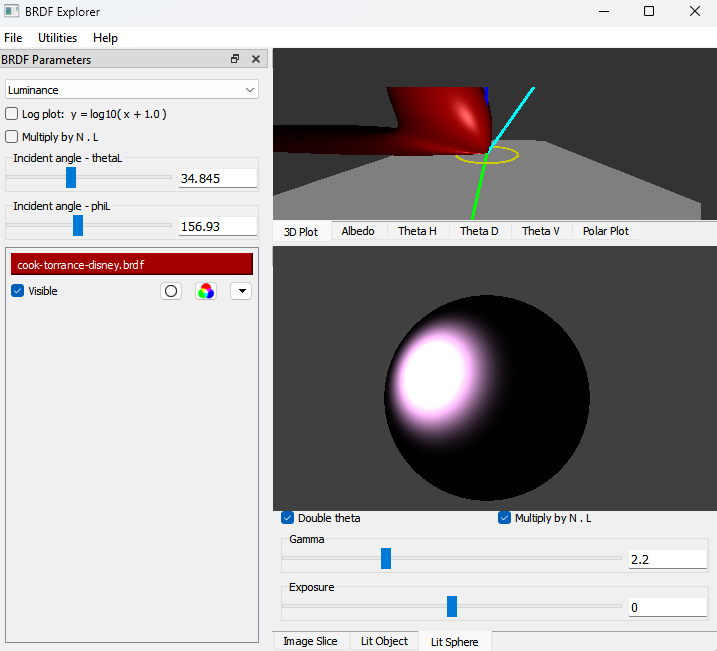
\includegraphics[width=0.65\textwidth]{./Imagens/disney-brdf-tool-original2.png}
           % \caption{\small Interface do Disney BRDF Explorer}
       \end{figure}

% \begin{lstlisting}[basicstyle=\tiny,language=C]
% ::begin parameters
% float n 1 1000 100
% ::end parameters
% ::begin shader
% vec3 BRDF(...) {
%    // código gerado
% }
% ::end shader
% \end{lstlisting}
    \end{columns}
\end{frame}
